%----------------------------------------------------%
%                    INTRODUCCION                    %
%----------------------------------------------------%

\pagestyle{fancy}

\chapter{Introducción}
\label{introduccion}

\section{Contexto}

Muchas veces nos encontramos con aulas con demasiados alumnos. Estas clases son especialmente comunes en los primeros cursos de los estudios universitarios, donde el número de alumnos alcanza fácilmente las tres cifras. Conocer todos los alumnos que tienen dudas y monitorizar a los alumnos para saber si todos o la mayoría han acabado el ejercicio son tareas difícilmente abordables por una sola persona. La mayoría de las veces se suelen ignorar los problemas y dudas, y se sigue adelante.\\

Los nuevos planes de estudio, que pretenden dejar atrás el sistema de educación mediante clases magistrales y dinamizar las clases, han supuesto un aumento en el número de clases prácticas y laboratorios que se realizan. Algunos centros han optado incluso por dividir las clases en grupos más pequeños para realizar las prácticas, pero muchas veces ésto no es posible. En esas situaciones el profesor acaba por no poder monitorizar completamente la clase.\\

Con el fin de tener un medio común se han implantado en los últimos años nuevas tecnologías en entornos docentes. Sin embargo, en muchos casos esta tecnología se limita a entornos de apoyo a la docencia más que al alumnado, siendo muy popular el sistema de gestión del aprendizaje Moodle. Además, el uso más frecuente de estos sistemas es el de simples almacenes de recursos bibliográficos (enlaces, apuntes, transparencias, etc.).\\

Por otro lado, la expansión de las tecnologías móviles y tabletas, con las que los alumnos están cada vez más familiarizados, no ha sido aprovechada. Estas tecnologías están ya mayoritariamente presentes en las aulas, la mayoría del alumnado dispone de alguno de estos dispositivos, pero su uso como herramienta educativa no es real, desperdiciando así todo su potencial como sistema de ayuda al aprendizaje. Es más, muchas veces el uso de estos dispositivos está prohibido o limitado en clase.\\

\section{Propuesta}

Nuestra propuesta pretende modificar y actualizar los modelos educativos presenciales a través de herramientas que faciliten la captura de la información de lo que sucede en el aula, con el objetivo de proporcionar \textit{feedback} a profesores y estudiantes sobre su progreso en el aprendizaje. Esta propuesta se materializa en la aplicación \textit{PresenceClick} que facilita la captura colaborativa de esta información entre alumnos y profesores de manera ágil.\\

\textit{PresenceClick} es un entorno modular colaborativo que facilita el registro en tiempo real de la información sobre los alumnos en sesiones tradicionales de aprendizaje con el propósito de obtener feedback de ayuda para mejorar el proceso de enseñanza aprendizaje.\\ 

\textit{PresenceClick} está compuesto por un sistema web (\textit{webClick}), una aplicación móvil (pClick) y un servidor de datos para mantener el modelo del Alumno y el modelo de Grupo (\textit{Learner and Group Models}). Ambas plataformas son a su vez modulares, dividiéndose así en diversos módulos encargados de las distintas interacciones que se registran en clase. La plataforma \textit{pClick} captura las interacciones de aprendizaje en tiempo real. Por otra parte, \textit{webClick} controla y muestra la información capturada durante sesiones cara a cara y permite a profesores y estudiantes seguir el progreso de sus alumnos durante el curso mediante visualizaciones y sus características \textit{web responsive} permiten su acceso desde cualquier dispositivo, por ejemplo: PC, portátiles, tabletas o \textit{smartphones}. La información capturada e integrada en los modelos de Alumno y de Grupo permite a profesores y estudiantes visualizar las actividades, conocimiento y comportamiento de estos. Este entorno cubre principalmente dos objetivos: mostrar a los profesores el estado de aprendizaje de sus alumnos y otras características para ayudarlos a adaptar sus estrategias de enseñanza; y mostrar a los alumnos su propio progreso y su comparación al grupo para promover un estado de reflexión que les permita mejorar su aprendizaje.\\

Actualmente, el Modelo Interacciones de \textit{PresenceClick} incluye varios tipos de interacciones: de gestión (asistencia, evaluaciones), de actividad (preguntas de profesores y respuestas de alumnos), emocionales (sensaciones de los alumnos mientras realizan actividades de aprendizaje) y de comportamiento (participación, actividad).\\

La figura \ref{fig:presenceclick-architecture} muestra las líneas de interacción en la arquitectura de \textit{PresenceClick}: (1) los asistentes comunican su presencia en clase al modelo del alumno a través de dispositivos de control de presencia, (2) profesores y estudiantes capturas las interacciones que realizan mediante \textit{pClick}, y (3) los profesores y estudiantes interactúan con \textit{webClick} para obtener información sobre el progreso del estudiante y del grupo.\\

\noindent
\begin{figure}[!htbp]
\noindent
\makebox[\textwidth][c]{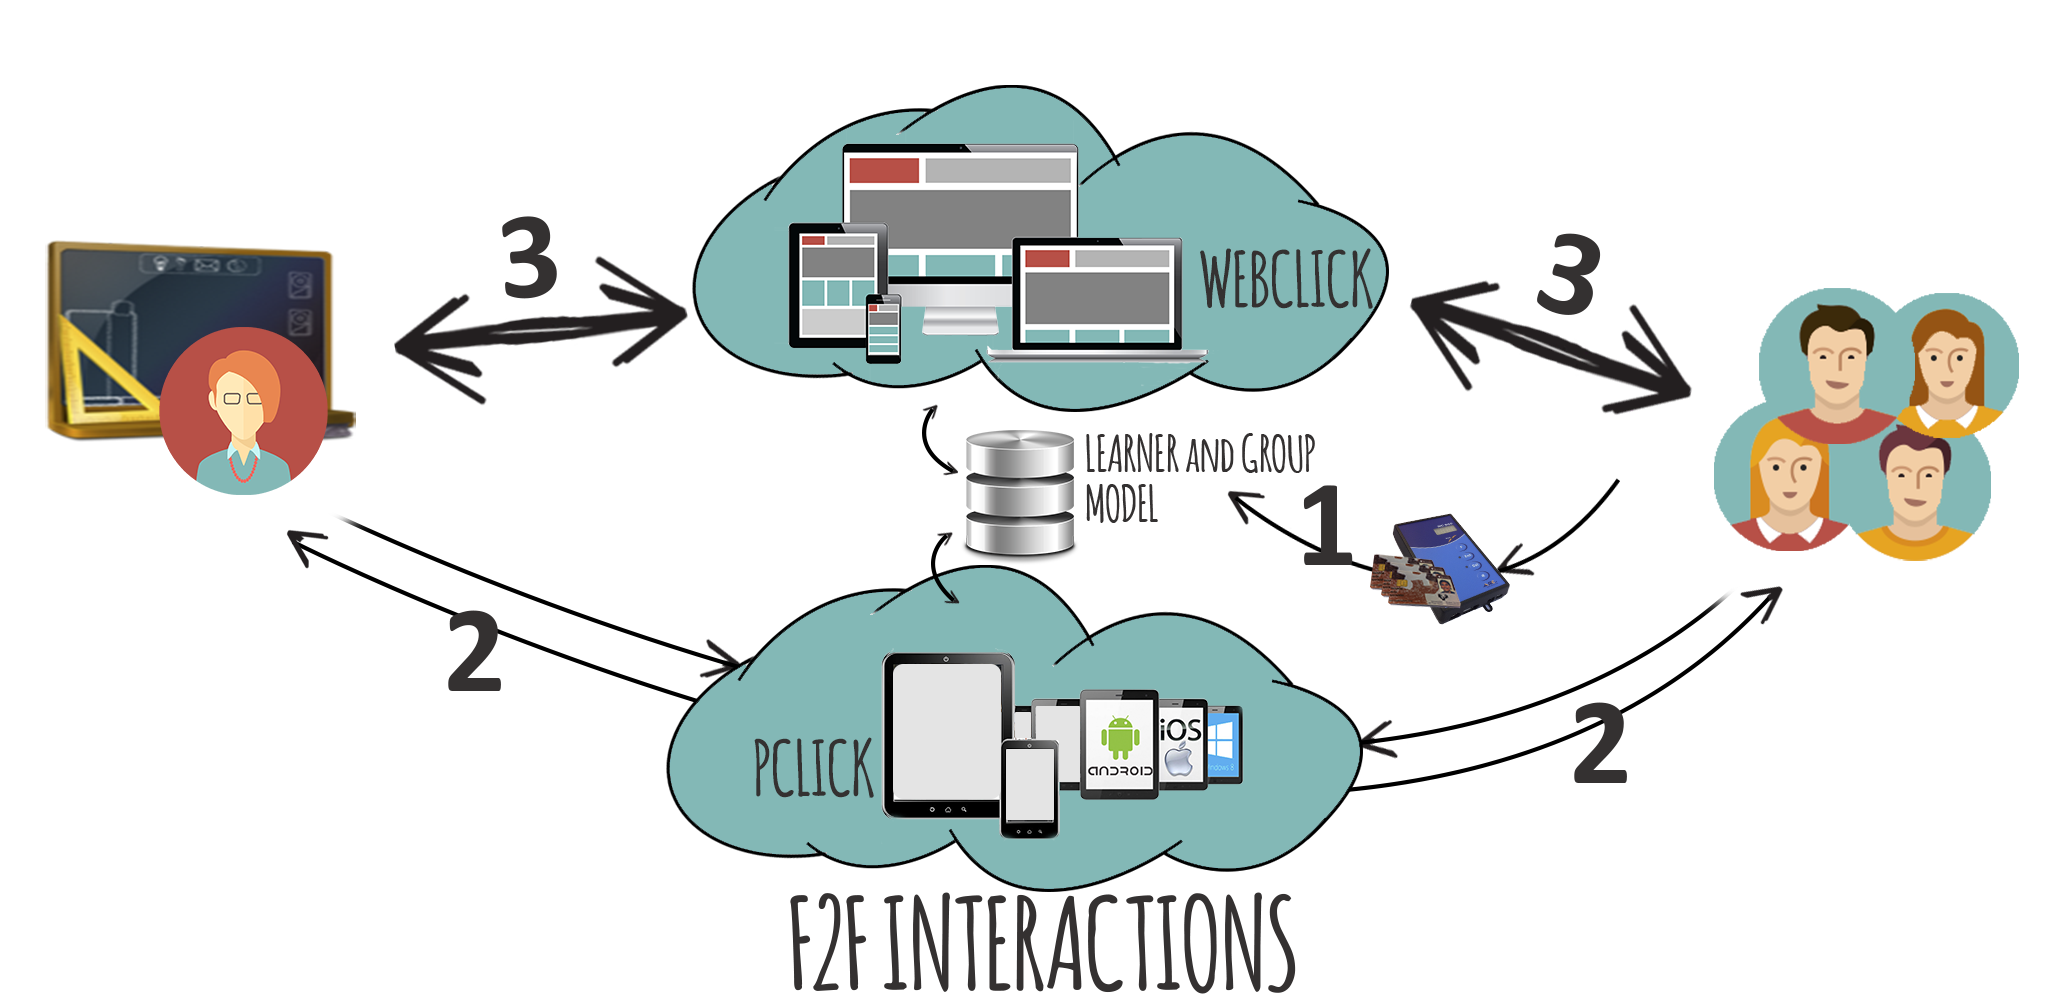
\includegraphics[width=\textwidth,keepaspectratio]{architecture}}
\caption{Arquitectura de \textit{PresenceClick}}
\label{fig:presenceclick-architecture}
\end{figure}

Actualmente pClick cuenta con un módulo llamado \textit{qClick} \cite{qclick}: un sistema de Pregunta-Respuesta en el aula, en el que el profesor lanza una pregunta a los alumnos y ellos a través de sus móviles pueden contestar a esa pregunta. Los resultados visualizados de forma gráfica a las preguntas realizadas pueden mostrarse a los alumnos en tiempo real. Este sistema permite motivar el debate en clase, bien antes de lanzar la pregunta para que discutan entre ellos las posibles respuestas o bien después de responderlas observando los resultados de la clase.\\

En este proyecto, nuestro objetivo es crear \textbf{un nuevo módulo de \textit{pClick} para capturar las interacciones entre profesor-alumnos en sesiones de ejercicios}. Por el momento se desarrollará como una aplicación independiente y más tarde se integrará en \textit{pClick}.\\

En esta aplicación el profesor dispondrá de una interfaz a la que accederá mediante su dispositivo móvil o tableta en clase e indicará a sus alumnos los ejercicios a realizar (está actividad se podrá planificar previa a la clase). Por su parte, los alumnos (que tienen que haber fichado con su tarjeta de alumno para entrar en clase) con sus dispositivos móviles (smartphones o tabletas) recibirán las notificaciones de los ejercicios a realizar y podrán indicar para cada uno si tienen dudas en su realización o si lo han terminado. El profesor podrá disponer en tiempo real de información sobre el porcentaje de alumnos que lo han realizado, alumnos que indican problemas en su realización y aquellos alumnos que no indican nada. Además el profesor podrá acercarse a comprobar y revisar las soluciones de los alumnos que indican haber terminado el ejercicio, y valorar su nivel de corrección o satisfacción en la realización, añadiendo las notas oportunas en el sistema que le permitirá seguir la evolución de cada uno de sus alumnos durante el curso. También podrá acercarse a aquellos que señalan problemas en su realización, con el fin de ayudarlos y evitar dificultades en su progreso.\\

Bajo este contexto surge \textbf{exerClick}, la herramienta para seguimiento de ejercicios en el aula. Esta herramienta, con todas sus funcionalidades, nace con el propósito de tener una visión más real de lo que hacen los alumnos, tanto una visión global del grupo como una individual y está dirigida a profesores y a los propios alumnos. De esta manera, el docente puede ofrecer un aprendizaje más adaptado e individualizado, aunque los grupos de alumnos sean muy grandes.\\

\section{Organización del documento}

En esta memoria se ha documentado  el desarrollo de la herramienta \textbf{\textit{exerClick}}, dentro del Trabajo de Fin de Grado (TFG) del autor. En el documento se describe la propuesta, la planificación y gestión que esta lleva consigo, la implementación llevada a cabo y las conclusiones finales.\\

En este primer capítulo se ha introducido el problema a resolver y se ha explicado la propuesta presentada en este proyecto.\\

En el capítulo 2 se presenta el Documento de Objetivos de Proyecto (DOP). Este recoge el alcance y las fases y tareas del proyecto, el análisis de riesgos y el análisis de factibilidad.\\

Una vez en el capítulo 3 se explica la gestión llevada a cabo durante el proyecto. Se presentan las metodologías utilizadas: Metodologías Ágiles e InterMod (adaptada a las necesidades de este proyecto). A continuación se detallan cada una de las iteraciones llevadas a cabo (como parte de la metodología InterMod): duración, objetivos y tareas realizadas. Al final del capítulo se muestra la documentación asociada a las iteraciones y los objetivos, además del seguimiento de tiempo realizado.\\

A continuación, en el capítulo 4 se detalla el análisis de requisitos. Primero se detallan los requisitos no-funcionales y luego los funcionales (prototipos en papel llevados a cabo durante las primeras iteraciones que dan una visión global del proyecto).\\

En el capítulo 5 se explica el diseño e implementación llevados a cabo. Se comienza mostrando la estructura de documentos del proyecto, luego el diseño realizado en base al análisis de requisitos del capítulo 4 y finalmente una visión general de la implementación de la lógica de negocio.\\

Para finalizar, en el capítulo 6 se presentan las conclusiones, líneas futuras para el proyecto y las lecciones aprendidas.\\

Fuera de la estructura general de la memoria, tenemos la bibliografia y los apéndices. En estos últimos tenemos las actas de reuniones, las actas de pruebas y la vista de relaciones de la base de datos (de la parte utilizada o creada específicamente para el proyecto).\\